%!TEX root = ../dissertation.tex
\begin{savequote}[75mm]
A man who procrastinates in his choosing will inevitably have his choice made for him by circumstance.
\qauthor{Hunter S. Thompson}
\end{savequote}

\chapter{The Large Hadron Collider}

\paragraph{}
The Large Hadron Collider (LHC) is a proton-proton collider at the European Organization for Nuclear Research (CERN) laboratory in Geneva, Switzerland~\cite{LHCPaper}. In order to discover the Higgs boson, the two most important design parameters for a collider are beam energy and luminosity. This chapter will cover how these two parameters are reached by the LHC, and the final design and layout.

\section{Beam Energy}
\paragraph{}
In order to probe the quarks and gluons inside, protons need to be accelerated to high energies. For a charged particle, charge $Z$ (for protons, $Z=1$) and momentum $p$, its trajectory within a magnetic field $B(s)$ is described by the deflection angle $d\theta$, with radius $\rho$.
%(See this \href{https://indico.cern.ch/event/626458/contributions/2529616/attachments/1434511/2205263/LHC-Ecal.ATLAS-plenary.Mar17.pdf}{talk}):
%
\begin{equation}
d\theta = \frac{ds}{\rho} = \frac{ZB(s)ds}{p}
\end{equation}
Integrate this angle over the circumference:
\begin{equation}
\oint_C d\theta = 2\pi = \frac{1}{p} \oint_C B(s)ds
\end{equation}
Thus the momentum ($\sim$ energy) of the charged particle is:
\begin{equation}
\label{Ch2:eq-p}
p = \frac{1}{2\pi}\oint_C B(s)ds = 1 \times 47.7[\frac{MeV}{cTm}] \oint_C B(s)ds
\end{equation}
%
\paragraph{}
In order to achieve a designed center of mass energy of $\sqrt{s} = 14 \TeV$, the momentum of the proton is $7$ \TeV. The Niobium Titanium magnetic dipole is $14.3$ meters in length, and while cooled by superfluid helium to a temperature of $1.9$ Kelvin, can generate $8.33$ Tesla magnetic field. Therefore, according to Eq\ref{Ch2:eq-p}, the LHC needs 1232 such magnets for steering. Additionally, 6800 superconducting magnets are used to focus the beam, squeeze the beam, correct the trajectory, and damp oscillation in beam position.


\section{Luminosity}
\paragraph{}
In order to study certain physics processes, the production rate affects the length of the experiment. The rate of a specified physics process $R_{\rm phy} = L\sigma$, where $L$ is the instantaneous luminosity ($m^{-2}s^{-1}$) the collider, and $\sigma$ ($m^2$) the physics process' cross section. The instantaneous luminosity is could be controlled and affects the experiment data taking length. For a Gaussian beam profile, it is defined in Eq\ref{Ch2:eq-lumi} ~\cite{LHCReview}:
%
\begin{equation}
\label{Ch2:eq-lumi}
L = \frac{N_b^2 n_b f_{\rm rev} \gamma_r}{4\pi \epsilon_n \beta^*} F
\end{equation}
%
In the above Eq\ref{Ch2:eq-lumi}:
\begin{itemize}
	\item $N_b$ is the number of protons per bunch; 
	\item $n_b$ is the number of bunches per beam; $n_b$ cannot be too large due to potential beam loss damages on the accelerator and detector; %Nominally, $2808$ proton bunches. 
	\item $f_{\rm rev}$ is the proton revolution frequency; or the ratio of the circumference of LHC, 26.7 km, and the speed of light.
	\item $\gamma_r$ is the relativistic Lorentz factor for the protons;
	\item $\epsilon_n$ is the average beam spread in the transverse plane;
	\item $\beta^*$ is a measure of the beam spread in the longitudinal direction; affected by focusing magnets;
	\item $F$ is a reduction factor for the angle beams are colliding; smaller crossing angles could cause larger spread in the longitudinal direction.
\end{itemize}

\paragraph{}
The instantaneous luminosity can also be written as the ratio of the rate of inelastic collisions to the inelastic cross section $\sigma_{\rm inel}$ ~\cite{lumi-paper}. 
\begin{equation}
\label{Ch2:eq-lumi2}
L = \frac{R_{\rm inel}}{\sigma_{\rm inel}} = \frac{\mu n_b f_{\rm rev}}{\sigma_{\rm inel}}
\end{equation}
where, $\mu$ is the number of interactions per bunch crossing. At each bunch crossing, multiple proton-proton collide, and the collisions without the highest center of mass energy are called ``pileup" interactions. The averaged collision activities over all bunch crossings, $\langle \mu \rangle$, is a measurement of the level of pileup in the detector. For High Luminosity LHC, the expected $\langle \mu \rangle$ is 200. The higher number of pileup, the higher total collision events are produced, but is harder for the detectors to distinguish each collision separately.


\paragraph{}
The target peak instantaneous luminosity for both the ATLAS and CMS experiments is $L=10^{34}~\text{cm}^{-2}\text{s}^{-1}$~\cite{LHCPaper}, which is already exceeded in 2016. The main parameters of the LHC beam and performance are shown in Table~\ref{Ch2:tab-lhc}. At the nominal LHC conditions, the beam energy is about 360 MJ, and the LHC in total consumes 115 MW of energy. 

\begin{table}[]
\centering
\begin{tabular*}{\textwidth}{@{\extracolsep{\fill}}llll}
\hline
Parameter [unit]   & Nominal design value & 2015 Operating value  & 2016 Operating value\\
\hline\hline
Beam Energy [TeV]  & $7$  & $6.5$  & $6.5$  \\
Peak L [$\text{cm}^{−2}~\text{s}^{-1}$]   & $10^{34}$ &   $5 \times 10^{33}$  & $1.25 \times 10^{34} $           \\
Bunch spacing [ns]             &      $25$  &  $25$ &      $25$ \\
$n_b$  [$10^{11}$ p/bunch]   & $1.15$ &  $1.15$ & $1.12$\\
$N_b$  [bunch]         & $2808$   &      $1825$ &      $2220$\\
$f_{\rm rev}$ [kHz]    &     $11245$  & $11245$  & $11245$ \\
$\epsilon_n$  [mm mrad]        & $3.5$ &  $3.5$  & $2$\\
$\beta^*$   [cm]         & $55$  &   $80$-$40$  & $40$\\
$F$        &      $0.84$  & $0.84$  &  $0.59$ \\
$\langle \mu \rangle$ & $19$ & $13$ & $41$ \\ \hline
\hline            
\end{tabular*}
\caption[LHC nominal and operational parameters]{LHC nominal~\cite{LHCPaper} and operational parameters in 2015~\cite{LHC_2015} and 2016~\cite{LHC_2016}.}
\label{Ch2:tab-lhc}
\end{table}

\section{Layout}
\paragraph{}
Protons accelerated in the LHC originate from a red bottle of hydrogen gas. The whole series take around 4 + 20 (LHC only) minutes:
\begin{itemize}
\item An electric field strips the electrons from the hydrogen to create protons; 
\item A linear particle accelerator, Linac 2, accelerates the protons to 50 MeV; 
\item The Proton Synchrotron Booster (PSB) accelerates the protons to 1.4 GeV;
\item The Proton Synchrotron (PS) accelerates the protons to 25 GeV; 
\item The Super Proton Synchrotron (SPS) accelerates the protons to 450 GeV; it sends the protons in bunch trains;
\item The LHC accelerates the protons in a series of Radio Frequency cavities to the final TeV energies.
\end{itemize}
Interaction points (IP) are where the two proton beams focused and collided. Only a part of the protons in the bunch collide, and the rest remains in LHC and travels to the next interaction point. 

\paragraph{}
ATLAS (A Toroidal LHC ApparatuS), CMS (the Compact Muon Solenoid), ALICE (A Large Ion Collider Experiment), and LHC$b$~\cite{ATLASPaper, CMSPaper, LHCbPaper, ALICEPaper} are the four main experiments. They are located at the IPs of the accelerator. Figure~\ref{fig:LHC} shows a schematic of the LHC ring and its experiments. 

\begin{figure}[h!]
  \centering
  \captionsetup{justification=centering}
  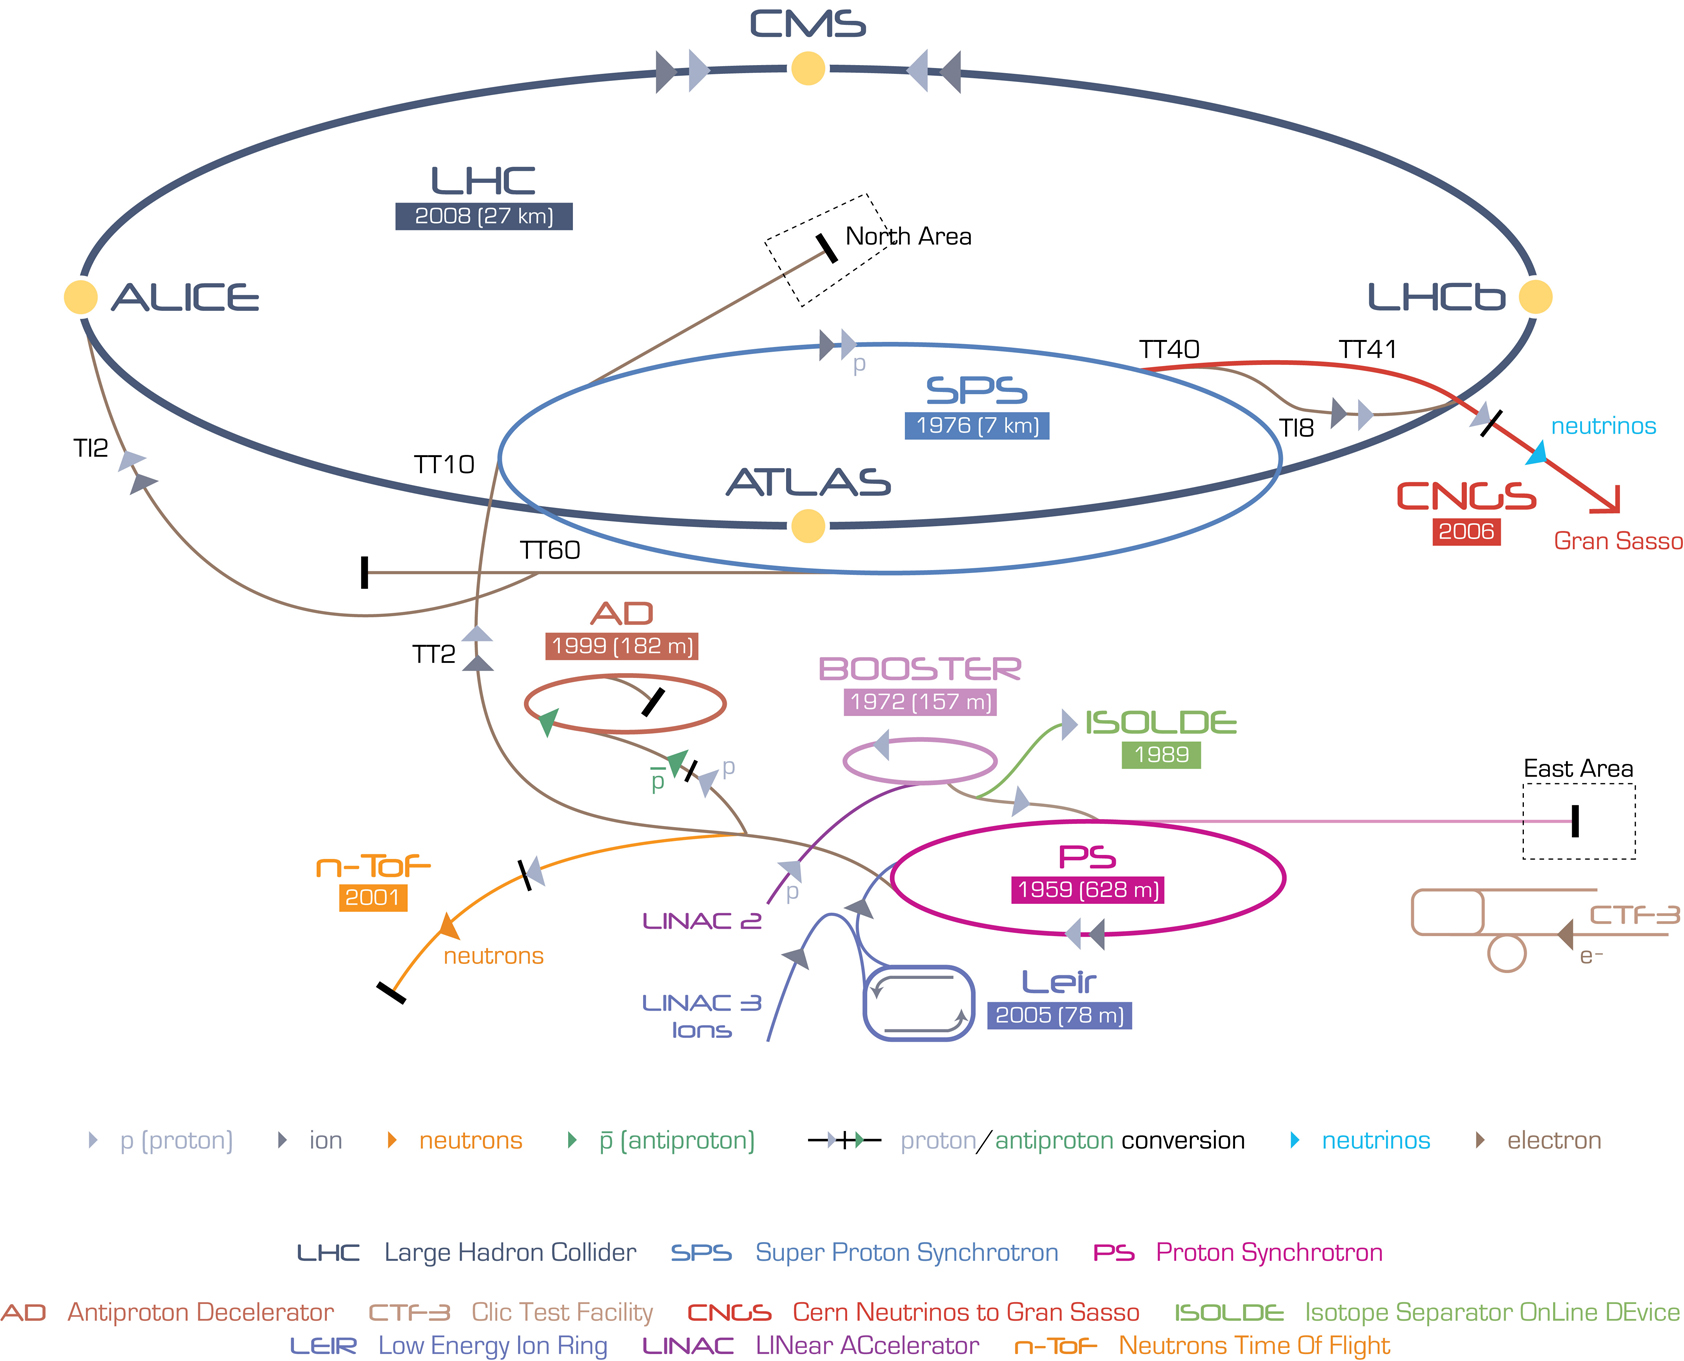
\includegraphics[width=0.7\textwidth]{figures/detector/Cern-Accelerator-Complex.jpg}
   \caption{A schematic view of the LHC ring~\cite{LHCReview}. LINAC2, Booster, PS, SPS, and LHC accelerate the protons in order. Four main experiments are located at interaction points along the ring. ATLAS and CMS are general purpose experiments, while ALICE focuses on heavy ion collisions and LHC$b$ is dedicated to $B$ physics.}
  \label{fig:LHC}
\end{figure}

% \paragraph{} 
% Above injection energy the relative beam energy uncertainty is $0.1\%$, fully correlated between the 2 beams. No correction must be applied to the online energy values. Energy and uncertainty are determined by the magnetic model, see \href{https://indico.cern.ch/event/626458/contributions/2529616/attachments/1434511/2205263/LHC-Ecal.ATLAS-plenary.Mar17.pdf}{talk}.